\documentclass[12pt]{article}

\usepackage {preamble}

\begin{document}

\author{}
\title{Материалы для подготовки к зачёту по ОС 2026}
\date{}
\maketitle
\tableofcontents


\newpage
\section{Практики}

\subsection{Базовые команды терминала Linux}

\begin{itemize}
	\item \textit{reset} "--- сброс настроек терминала (например, если сломалась кодировка);
	\item \textit{clear} или \textit{Ctrl+L} "--- очистка экрана терминала;
	\item \textit{strings <бинарный файл>} "--- вывод всех текстовых строк, содержащихся в бинарном файле;
	\item \textit{set} "--- список всех системных переменных;
	\item \textit{ln myfile myfile.hard} "--- создание жёсткой ссылки (только в пределах файловой системы);
	\item \textit{ln "="=symbolic ("=s) myfile myfile.sym} "--- создание символической ссылки (может вести на несуществующий файл, аналогично ярлыкам);
	\item \textit{file <файл>} "--- информация о файле (empty/ASCII string/binary file и т.д.);
	\item \textit{which <команда>} (например, \textit{which bash}) "--- информация о расположении бинарного файла команды;
	\item \textit{mkdir "=p dir1/dir2/dir3} "--- создать иерархическую структуру директорий, все несуществующие директории на пути также будут созданы;
	\item \textit{rmdir dir1} "--- удалить пустую директорию;
	\item \textit{rm "=r dir1} "--- удалить директорию вместе со всем её содержимым;
	\item \textit{ls {>} file.txt} "--- перенаправление вывода в файл (если он уже существовал, то он будет перезаписан);
	\item \textit{ls {>}{>} file.txt} "--- перенаправление вывода в файл (если он не существовал, то он будет создан, иначе добавление производится в конец существующего файла);
	\item \textit{history} "--- история команд (можно выполнять навигацию с помощью $\uparrow$ и $\downarrow$);
	\item \textit{kill "=n <signum> <pid>} "--- послать сигнал с номером \textit{signum} процессу \textit{pid};
	\item \textit{ps "=ef} "--- диспетчер задач.
\end{itemize}

\subsection{Синонимы для директорий}

\begin{itemize}
	\item $\sim$ "--- домашняя директория;
	\item $\sim$ <username> "--- домашняя директория пользователя \textit{username} (/home/username);
	\item . "--- текущая директория;
	\item .. "--- родительская директория.
\end{itemize}

\subsection{Мануалы}

\begin{figure}[H]
	
\includegraphics{man.jpg}
\end{figure}

Самое важное "--- это ЧИТАТЬ МАНЫ.

\begin{itemize}
	\item \textit{man <команда>} "--- ман по команде;
	\item \textit{man "=k <слово>} или \textit{apropos (appropriate position) <слово>}"--- все страницы манов, где встретилось слово;
	\item \textit{<команда> "="=help} или \textit{<команда> "=h} "--- для простых смертных, краткая справка по команде.
\end{itemize}

\subsection{Работа с правами файлов}

\textit{ls "=l} выводит подробную информацию обо всех файлах вместе с их флагами.

Пример флага: "=rwx"=wx"=w"=

Подробный разбор флага:
\begin{enumerate}
	\item Первый символ отвечает за то, является ли файл специальным (для директории там будет стоять $d$, для символической ссылки "--- $l$, для обычного файла "--- прочерк ("=)).
	\item Следующие три символа (с 2 по 4) отвечают за права владельца.
	\item Следующие три символа (с 5 по 7) отвечают за права группы.
	\item Последние три символа (с 8 по 10) отвечают за права остальных пользователей.
\end{enumerate}

\begin{itemize}
	\item $r$ (Read) "--- право записи;
	\item $w$ (Write) "--- право чтения;
	\item $x$ (eXecute) "--- право исполнения;
	\item "= (прочерк) "--- такого права нет.
\end{itemize}

\textit{chown <user> <file>} "--- передать права владения файлом пользователю user.

\textit{chmod u=rwx, g--x, o+rw <file>} "--- дать владельцу все права, у пользователей группы забрать права на исполнение, а остальным пользователям добавить возможность читать файл и писать в него.

Флаг можно закодировать как двоично"=десятичное число. Например, флаг rwx"="=x"=wx будет закодирован как $111_2 001_2 011_2 = 713_{10}$.

\textit{chmod 777 <file>} "--- дать на файл все права всем пользователям.


\newpage
\section{Программы с практических занятий (за работоспособность не отвечаю)}

\subsection{Лесенка из звёздочек на bash}
\inputminted{bash}{star_ladder.sh}

\subsection{Hello World}
\inputminted{c}{hello_world.c}

\subsection{Hello World с количеством повторений, заданным в аргументах командной строки}
\inputminted{c}{hello_world_with_arguments.c}

\subsection{Вывод аргументов командной строки}
\inputminted{c}{arguments_list.c}

\subsection{Лесенка из звёздочек и точек}
\inputminted{c}{star_ladder.c}

\subsection{Зеркальная лесенка из звёздочек и точек}
\inputminted{c}{star_triangle.c}

\subsection{Перевод числа из двоичной в десятичную систему счисления}
\inputminted{c}{to_dec.c}

\subsection{Сложение двоичных чисел}
\inputminted{c}{add_bin.c}

\subsection{Умножение двоичных чисел}
\inputminted{c}{mul_bin.c}

\subsection{Получение текущей даты}
\inputminted{c}{timestamp.c}

\subsection{Шифр Цезаря (probably doesn't work)}
\inputminted{c}{encode.c}

\subsection{Непрерывная запись в файл}
\inputminted{c}{continous_write_to_file.c}

\subsection{Непрерывная запись в файл с использованием дочернего процесса}
\inputminted{c}{continous_write_to_file_with_fork.c}

\subsection{Непрерывная запись в файл с помощью демона}
\inputminted{c}{daemon.c}

\subsection{Самодельный аналог cp}
\inputminted{c}{copy.c}

\subsection{Простой обработчик сигналов}
\inputminted{c}{simple_signal_handler.c}

\subsection{Продвинутый обработчик сигналов}
\inputminted{c}{advanced_signal_handler.c}

\subsection{Самодельный аналог kill}
\inputminted{c}{kill.c}

\subsection{Информация о PID, PPID, SID, GRPID процесса}
\inputminted{c}{pid_sid_grp_info.c}

\subsection{Программа, автоматически меняющая свой PID и название}
\inputminted{c}{change_pid.c}


\newpage
\section{Лекции}

\subsection{Введение}

Компьютеры делятся на цифровые вычислительные машины (ЦВМ) и аналоговые вычислительные машины (АВМ). Планировщик распределяет время между процессами с помощью карусели/приоритетов, т.е. применяются квазипараллельные вычисления (в каждый момент времени процессор занят одной задачей, но эти задачи постоянно меняются).

Операционные системы делятся на универсальные ОС и ОС реального времени. Существуют однопользовательские и многопользовательские ОС. 

Сервис "--- подпроцесс, работающий самостоятельно и изолированный от других.

\subsection{История Unix}

Multics. Первая ОС, написанная на языке высокого уровня (\textbf{C}) "--- Unix. А. Танненбаум "--- Minix. Линус Торвальдс "--- Linux (монолитное ядро, в результате спора с Танненбаумом Linux остался обозначением для ядра, а не для полноценной ОС). FreeBSD. QNX (Quick Unix) "--- ОС реального времени с микроядерной архитектурой.

Linux "--- это только ядро, мы же пользуемся \textit{дистрибутивами} Linux. Дистрибутив включает в себя ядро, пакетный менеджер и набор прикладных программ.

\begin{figure}[H]
	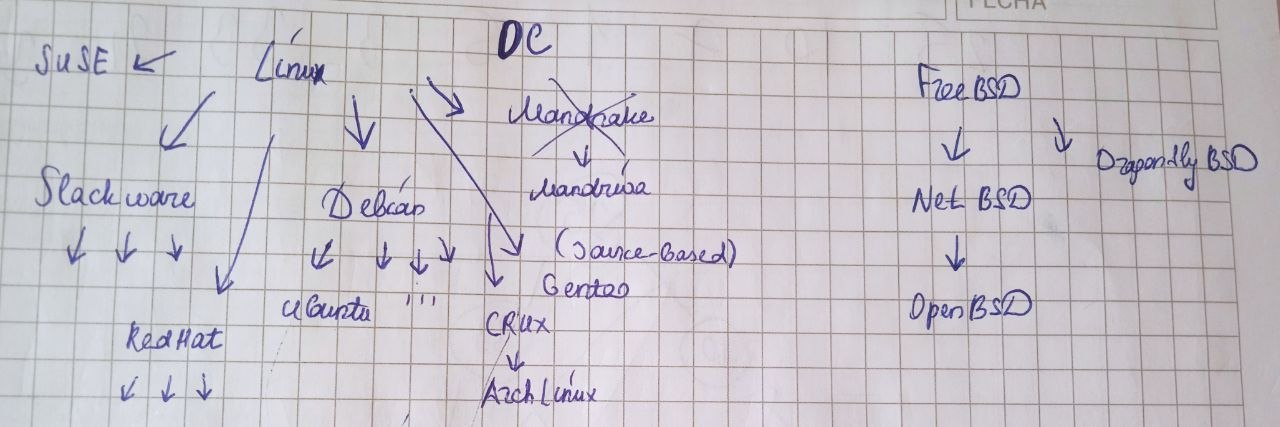
\includegraphics[scale=0.4]{linux_distributions.jpg}
	\centering
	\caption{Схема дистрибутивов Linux и FreeBSD}
\end{figure}

LFS "--- Linux From Scratch, возможность создать собственный дистрибутив.

LSB "--- Linux Standard Base.

SUS "--- Single Unix Specification.

\subsection{Компьютерные сети}

Коммутация каналов/коммутация пакетов.

Протокол "--- соглашение по передаче"=обработке данных.

RFC "--- requests for comments.

\begin{figure}[H]
	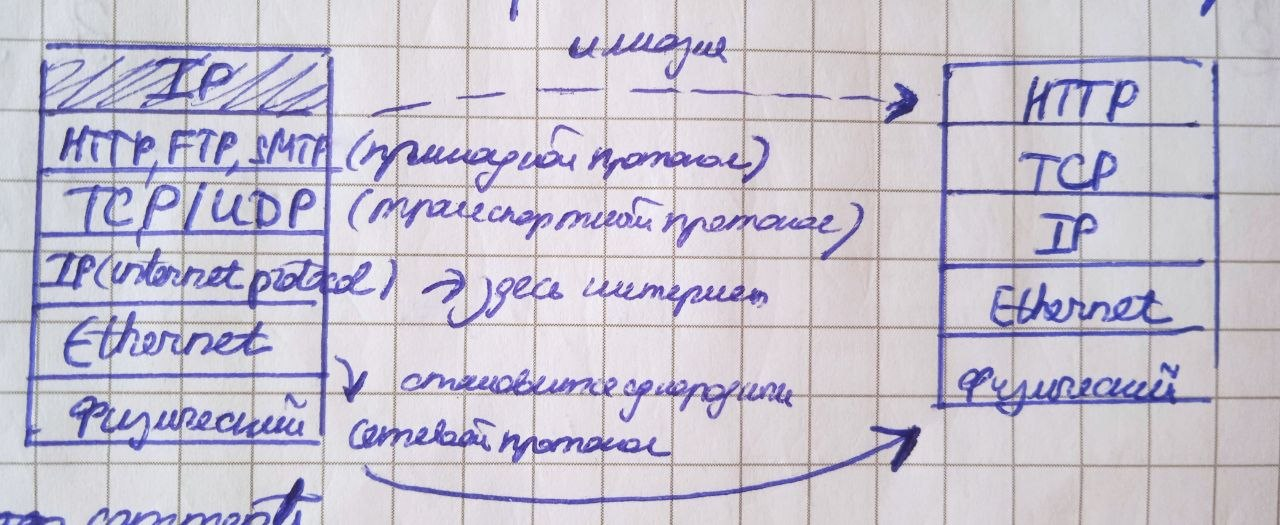
\includegraphics[scale=0.4]{protocols.jpg}
	\centering
	\caption{Стек протоколов}
\end{figure}

\subsection{Уровни операционной системы}

\begin{enumerate}
	\item Kernel "--- ядро, внутренний уровень;
	\item Shell "--- оболочка, внешний уровень.
\end{enumerate}

X Window System "--- графическая оболочка.

XLog "--- окно входа X Server.

\subsection{Системные вызовы}

Аналог команды cp с помощью высокоуровневых функций работы с файлами:

\begin{minted}{c}
FILE* fv = fopen("from.txt", "r");
FILE* tv = fopen("to.txt", "w");
while ((c = getc(fv)) != EOF) putc(c, tv);
fclose(fv);
fclose(tv);
\end{minted}

Системные вызовы для работы с файлами:

\begin{itemize}

\item Создание файла:
\begin{minted}{c}
creat("file.txt", 0642);
\end{minted}

\item Сброс прав по умолчанию:
\begin{minted}{c}
umask(0);
\end{minted}

\item Создание файла и запись в него:
\begin{minted}{c}
char buf[10];
umask(0);
int fd = creat("file.txt", 0642);
write(fd, buf, sizeof(buf));
close(fd);
\end{minted}

\item Открытие файла (старый способ):
\begin{minted}{c}
int mode = 1; // 0 - r, 1 - w, 2 - rw
open("file.txt", mode);
\end{minted}

\item Открытие файла (новый способ):
Применяются флаги, их можно комбинировать через побитовое или (|).
\begin{enumerate}
	\item O\_CREAT "--- создать;
	\item O\_RDONLY "--- открыть только для чтения;
	\item O\_WRONLY "--- открыть только на запись;
	\item O\_RDWR "--- открыть на чтение и запись;
	\item O\_APPEND "--- запись в конец файла;
	\item O\_NDELAY "--- не блокировать при открытии;
	\item O\_TRUNC "--- сократить размер файла до нуля.
\end{enumerate}

\begin{minted}{c}
int fd = open("from.txt", O_RDONLY);
int to = open("to.txt", O_WRONLY | O_CREAT);
char buf[10];
while ((n = read(fd, buf, sizeof(buf))) > 0) {
	write(to, buf, n);
}
\end{minted}

\item Перенос указателя:
Сдвинуть указатель файлового дескриптора \textit{fd} на 3 байта вправо с начала:
\begin{minted}{c}
lseek(fd, 3, 0);
\end{minted}

\end{itemize}

Стандартные потоки: $0$ "--- stdin, $1$ "--- stdout, $2$ "--- stderr.

\end{document}
